\documentclass[11pt,a4paper,twocolumn]{book}
\usepackage[utf8]{inputenc}
\usepackage{tikz}
\usetikzlibrary{er,positioning}
\usepackage[english]{babel}
\usepackage{amsmath}
\usepackage{amsfonts}
\usepackage{array}
\usepackage{amssymb}
\usepackage{listings}
\usepackage{booktabs}
\usepackage{graphicx}
\usepackage{multirow}
\author{Ege Özkan}
\title{CENG315 \\ \large{Information Managment Lecture Notes}}
\begin{document}
\lstset{language=SQL}
\newcommand{\missing}{\textit{(!*)}}
\newcommand{\unsure}{\textit{?*}}
\newcommand{\code}[1]{\texttt{#1}}
\newcommand{\set}[1]{\ensuremath{\{ #1 \}}}
\newcommand{\join}{\ensuremath{\bowtie}}
\newcommand{\fd}[2]{$ \code{#1} \to \code{#2} $}
\newcommand{\assign}{\ensuremath{\leftarrow}}
\maketitle

\frontmatter

\tableofcontents

\section*{Editor's Note}

Within the book, there are some instances where a text is presented within square brackets. These are the Editor's Commentary, these may be thoughts that popped into my mind while taking notes, additional information or clarifications. Now, nothing in the book is guaranteed to be correct, but most of it is at least information I transcribed from an expert, so Editor`s Notes are extra likely to be wrong, enjoy.

\mainmatter
\chapter{Introduction - October 15, 2020}

\section{Databases and Database Systems}

Databases hold data. Database systems are software systems that manages the records in a database. There are five fundemental requirements for a database system.

\begin{itemize}
\item Database systems must be persistent, data must be storable and remain for the future.
\item Databases must be able to handle getting large.
\item Databases should be sharable, multiple users should be able to reach it at the same time.
\item Databases must be kept accurate.
\item Databases must be usable.
\end{itemize}

\subsection{Record Storage}

Databases can be made persistent in different ways.

\subsubsection{Storing database records in text files}

\begin{itemize}
\item Simplest approach.
\item One file per record type.
\item Each record could be a line of text, with its values seperated by tabs.
\end{itemize}

\begin{lstlisting}
1	joe	2020
2	amy	2013
3	lee	2000
\end{lstlisting}

Its advantages are the database system has to do very little, and a use could easily examine and modify the files with a text, but it is slow. \missing

\subsection{Data Models and Schema}

Data models are different ways to express connections between records while Schemas are the implementations of these methdos for a specific database.

\subsubsection{File-system v. Relational}

In the file system modal, each record type has a file, with one record per line, programs that read and write to the file is responsible for understanding this. In the relational data model, each record type has its \textbf{table} and each record has \textbf{fields} for each value. User access to the database happens via this record and field model and records that fit certain conditions can be quarried.\\

These models are at different levels of abstraction, relational model is a \textbf{conceptual model}, since there is no need to know \textbf{how} schemas are specified and implemented, the conceptual schema describes what the data \textit{is}. Whereas the file-system is called a \textbf{physical model}, physical schemas say how the data is \textit{implemented}.

\subsubsection{Physical Data Independence}

A conceptial schema is certainly nicer to use than a physical scheme. Operations on a conceptual schema is implemented by the database schema. Database system has a \textbf{database catalog} that contains descriptions of the physical and conceptual schemas. Givven an SQL querry, the database system translates the conceptual abstraction to the physical one and interract with it on the users behalf. If the user does not have to deal with the physical level, this is called the Physical Data Independence.

It is easy to use, quaries are optimized automatically and it is isolated from changes to the physical schema.

\subsubsection{Logical Data Independence}

The set of tables personalized for a particular user is called the user's \textbf{external schema}. If users can be given their own external schema in a database system, it is told that this Database System supports Logical Data Independence.\\

It has three benefits:

\begin{itemize}
\item Each users gets a customized external schema, they see only the information they need.
\item The user is isolated from changes to conceptual schema.
\item It is safer.
\end{itemize}

\section{Relational Databases}

The relational modal is a conceptual model since its schemas do not depend on the pyhsical level.

\subsection{Tables}

The database is organized into \textbf{tables}, which contain zero or more \textbf{records} (ie: table rows), and at least one \textbf{fields} (ie: the columns of the table.) Each record has a value for each field, and all fields has a specific \textbf{type}. Often, when discussing tables, the type information ignored.

\begin{figure}
\begin{lstlisting}
STUDENT(SId, SName, GradYear, MajorId)
DEPT(DId, DName)
COURSE(CId, Title, DeptID)
SECTION(SectId, CourseId, Prof, Year)
DEPARTMENT(DId, Name)
\end{lstlisting}
\caption{An example schema}
\label{schema:univesity}
\end{figure}

\subsubsection{Null Values}

A \texttt{null} value denotes a value that \textit{does not exist} or is \textit{unknown}. It occur if the data collection is incomplete or if data has not arrived yet.

\subsection{Superkeys and Keys}

In the relational model, the access to data is not handled by indices. Instead, a record must be referenced by specifying field values. Since not all values are guranteed to be unique for all users, a unique identifier field is called a \textbf{superkey} to distinguish it. Adding a field to a superkey, will generate another superket. A \textbf{key} is a superkey with the property that no subset of its fields is a super key.\\

\subsubsection{Primary Keys}

In the Schema at Figure \ref{schema:univesity}'s, \texttt{STUDENT} table \texttt{SId} is a key. Whereas in \texttt{SECTION} there may be multiple keys if each professor teaches only one class. Therefore, since a table may have multiple keys, a key is chosen as a \textbf{Primary Key}, whose  values \textit{should never be null}, and who is used to refeer to each record.\\

For instance, in Figure \ref{schema:univesity}, \texttt{STUDENT} table, \texttt{SId} can be the primary key. This is no coincidance, IDs are most times fit to be primary keys.

\subsubsection{Foreign Keys}

The information in a database is split among tables, these are not isolated from each other, a \textbf{foreign key} is a field (or fields) of one table which corresponds to the primary key of another table. For instance, in Schema at Figure \ref{schema:univesity}, \texttt{CourseId} of the \texttt{SECTION} table is a foreign key.\\

Foreign Keys can be used to create logical connections between different types of records. In the Schema at Figure \ref{schema:univesity}, \code{CourseId} of the \code{SECTION} table creates a logical connection between the \code{SECTION} table and \code{COURSE} table, since the objects these represent in real life, Sections and Courses are bound by a logical connection as well. (Each section is a section of a course).

\subsubsection{Foreign Keys and Referential Integrity}

The specification of a foreign key asserts \textbf{referential integrity}. Which requires each non-null foreign key value to be the key value of some record. Database system must ensure that if the primary keys of a table is modified in some ways, the foreign keys in other tables refeering to primary keys must also be updated accordingly, or set to \code{null} in worst case scenerio.

\subsection{Constraints}

A \textbf{constraint} describes the allowable states that fields can have in a table. There are four important kinds of constraints. \textbf{Null Value Constraints} limit fields to not have \code{null} values. \textbf{Key constraints} specify that two records cannot have the same value. \textbf{Referential integrity constraints} specify referential integrity, finally \textbf{integrity constraints}.

\subsubsection{Integrity constraints}

These constraints encodes \textit{business rules}. They can detect bad data entry and can enfore the \textit{rules} of the organization. They may apply to tables, individual records or the entire database.

\subsection{Table Specification in SQL}

\begin{lstlisting}[caption={the SQL specification of the STUDENT table},label={lst:student}]
create table STUDENT (
	SId int not null,
	SName varchar(10) not null,
	MajorId int,
	GradYear int,
	
	primary key (SId),
	foreign key (MajorId) references DEPT
		on update cascade
		on delete set null,
	check (SId > 0),
	check (GradYear >= 1863)
)
\end{lstlisting}

In Listing \ref{lst:student} we can see constraints and fields. The action specified with the \code{on delete} and \code{on update} keywords can be one of the following:

\begin{description}
\item[Cascade] causes the same query to apply to each foreign key record.
\item[Set null] causes the foreign key values to be set to null.
\item[Set default] causes the foreign key values to be set to their default value.
\item[No action] causes query to be rejectd if there exists and effected value with the foreign key.
\end{description}

\part{Theoretical Foundations \& Database Design}

\chapter{Relational Algebra - October 22, 2020}

\begin{table}[h]
    \centering
    \begin{tabular}{llll}
		ID & Name & Dept. Name & Salary\\
        \toprule
        22222 & Einstein & Physics & 95000\\
        12212 & Tesla & Physics & 4354\\
        \bottomrule
    \end{tabular}
    \caption{Instructors.}
    \label{tab:inst}
\end{table}

\section{Structure of Relational Databases}

Databases are structured with atrributes and values as tuples corresponding to those attributes.

\subsection{Attributes}
The domain of teh attribute is a set of allowed values. Attribute values are normally required to be \textbf{atomic}.

The \textbf{null} value is a special value that signifes that the value is unknown, or does not exist, it is a member of every domain. However, it causes complications.

\subsection{Schema vs Instance}

A database schema is the logical structure of the database. \texttt{instructor(ID, name, dept\_name, salary)}. A database instance is the snapshot of the database in a given time.

Using common attributes in relation schemas is one of \missing. There is also need for a \missing.

\subsection{Keys}

A \textbf{superkey} is a set of one or more attributes that allow us to identify uniquely a tuple in relation. Let $L \subset R$, superkey  $K$ is a \textbf{candidate key} if $K$ is minimal. One of the candidate keys is selected to be \textbf{primary key}, they should be chosen such that its attribute values are never or very rarely changed.\\

\textbf{Foreign key constraint} states that value in one relation must appear in another. \textbf{Referencing relation} is the relation that refeers to another and \textbf{Referenced relation} is the reference that is being referenced.

\section{Relational Query Languages}

A \textbf{query language} is a language in which a user requests infromation from the database. \textbf{Relational algebra} provides a set of operations that take one or more relations as input and return a relation as an output.

\section{Operations of Relational Algebra}

Relational algebra provides operations that take relations as input and returns relations as output.

\subsection{Select Operation}

Select operator selects $\sigma_p (r)$ (or \texttt{select(r, p)} to denote the selection of rows (horizontal selection) to denote selection on relation $r$ with respect to predicate $p$.\\

For instance, $\sigma_{A=B \land D>5}(r)$ would select tuples of relation $r$, such that its $A$ and $B$ attributes are equal and values of $D$ attribute is greater than 5\\

On the Table \ref{tab:inst}, $\sigma_{\text{dept\_name}=\text{"Physics"}(\text{instructor})}$ would return a tuple of instructors whose department is Physics.\\

Selection predicate can take comparasions using $=, \neq, >, \geq, <, \leq$ and multiple predicates can be combined using \textbf{connectives.} $\land, \lor$ and $\lnot$.\\

For instance on the department table with schema \texttt{department(dept\_name, building, budget)}, $\sigma_{\text{dept\_name}=\texttt{building}}(\text{department})$ would return departments whose names equal to their building's name.\\

\subsection{Project Operation}

An unary operation that returns its argument relation with certain attributes left out. $\Pi_{A_1, A_2, A_3, \dots, A_k}(r)$ or \texttt{project(r, {$A_1, A_2, A_3, \dots, A_k$})} where $A_n$ are attribute names and $r$ is a relation.\\

In essance project operation returns tuples with only the values whose attributes are listed in the operation.\\

\subsection{Composition of Relational Operations}

Since the result of a relational operation are itself a relations, operations can be given as input to other operations, ie: they can be composed together into a \textbf{relational-algebra expression}, finding the names ofa ll instructors in the physics department can be done by:

\begin{equation}
\Pi_{\texttt{name}}(\sigma_{\texttt{dept\_name} = \texttt{"Physics"}}(\texttt{instructor}))
\end{equation}

\subsection{Cartesian Product Operation}

Composes two relations together to a single product, $\texttt{instructor} \times \texttt{teaches}$ relation, where \texttt{instructor(id, name, dept\_name, salary)} and \texttt{teaches(id, course\_id, year} results in the relation \texttt{instructor$\times$teaches(instructor.id name, teaches.id, course\_id, year)}\\

However, as one can see, common attributes are not joined, therefore the cartessian product may not (and most likely will not) result in logical results.\\

When to attribute names are the same, they can be distinguished by attaching the name of the relation prior to the attribute name.\\

\subsection{Join Operation}

To avoid the mistake of illogical results, one can write:

\begin{equation}
\sigma_{\texttt{instructor.id}=\texttt{teaches.id}}(\texttt{instructor}\times\texttt{teaches}).
\end{equation}

The join operator is the equivalent of this expression. \textbf{Natural join} operation is denoted by $\join$ Outputs of the rows from the two input relations that have the same value on all atributes that have the same name is joined.\\

Consider relations $r$ and $s$, let $\theta$ be a predicate on attributes in the schema $r \cup s$. The join operation $r \join_\theta s$ is defined as $r \join_\theta s = \sigma_\theta (r \times s)$

Such as $\code{teaches} \join_{\code{teaches.id} = \code{instructor.id}}( \code{instructor})$ is equivalent to $\sigma_{\texttt{instructor.id}=\texttt{teaches.id}}(\texttt{instructor} \times \texttt{teaches})$

\subsection{Union Operation}

The union operation $r \cup s$ combines two relations as long as they have the same \textbf{arity} (number of attributes) and the attribute domains are compatible. (Same indexed attributes have the same domain.)\\

The expression $\pi_{\code{course\_id}}(\sigma_{\code{semester}=\code{"Fall"} \land \code{year} = 2017}(section) \cup \pi_{\code{course\_id}}(\sigma_{\code{semester} = \code{"Spring"} \land \code{year} = 2018}(section)$ on the relation \code{section} with schema \code{section(course\_id, sec\_id, semester, year, building, room, number, time\_slot\_id)} wil select \code{course\_id} row of the course that are though on Fall 2017 \textbf{or} Fall 2018.

\subsection{Set Intersection Operation}

Set intersection $s \cap r$ works exactly the same (and have the same assumptions.), but instead of working like \textit{or}, it works like \textbf{and}.

\subsection{Set Difference Operation} 

Set differnce $s - r$ works similar to intersection and union, but it selects those tuples that are on the first relation and \textbf{not} on the second relation.

\subsection{Rename Operation}

Given the relational algebra expression $E$, the expression $\rho_x(E)$ returns the expression $E$ under the name $X$.\\

It can also return an output whose attribute names are changed when they are listed $\rho_{x\{A_1, A_2, \dots, A_n\}}(r)$.

\subsection{Assignment Operation}

The assignment operation $\assign$ works like assignment in a programming language, relation algebra expressions can be assigned to temporary relation variables.

\begin{align*}
\code{Physics} \assign \sigma_{\code{dept\_name} = \code{"Physics"}}(\code{instructor})\\
\code{Musics} \assign \sigma_{\code{dept\_name} = \code{"Musics"}}(\code{instructor})\\
\code{Musics} \cup \code{Physics}
\end{align*}

\subsection{Equivalent Queries}

Since there is more than one way to write a query in relational algebra, queries that are not identical may be \textbf{equivalent}, they give the same result on any database.

\subsubsection{Alternative Notation}

On a related note, queries can be written with the alternative notation shown. For instance, \code{select(p, r)} instead of $\sigma_p (r)$

\chapter{Database Design - November 12, 2020}

\section{Design Phases}

\missing, First the database needs must be understood, after the database is designed conceptually. The final design is done in two phases, logical and phusical design, logical design is deciding on the schema, and phiscal design is choosing the implementation.

\section{Entity Relationship Model}
\scalebox{0.65}{
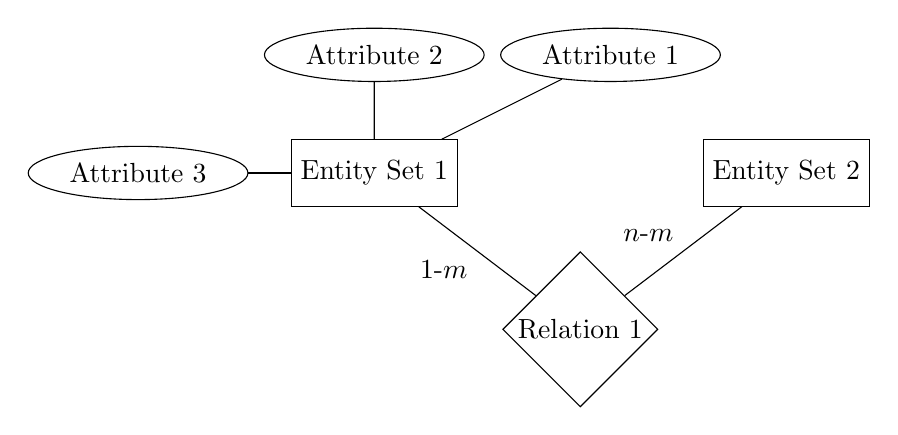
\begin{tikzpicture}[auto,node distance=1.5cm]
  % Create an entity with ID node1, label "Fancy Node 1".
  % Default for children (ie. attributes) is to be a tree "growing up"
  % and having a distance of 3cm.
  %
  % 2 of these attributes do so, the 3rd's positioning is overridden.
  \node[entity] (node1) {Entity Set 1}
    [grow=up,sibling distance=3cm]
    child {node[attribute] {Attribute 1}}
    child {node[attribute] {Attribute 2}}
    child[grow=left,level distance=3cm] {node[attribute] {Attribute 3}};
  % Now place a relation (ID=rel1)
  \node[relationship] (rel1) [below right = of node1] {Relation 1};
  % Now the 2nd entity (ID=rel2)
  \node[entity] (node2) [above right = of rel1]	{Entity Set 2};
  % Draw an edge between rel1 and node1; rel1 and node2
  \path (rel1) edge node {1-\(m\)} (node1)
    edge	 node {\(n\)-\(m\)}	(node2);
\end{tikzpicture}
}

Models and enterprise as a collection of \textbf{entities} and \textbf{relationships}. It is also called the ER diagram. It consists of three basic structures, \textbf{entity sets}, \textbf{relationship sets} and 

\begin{description}
\item[Entity] a thing or an object in the enterprise that is distinguishable from other objects, described by a set of \textit{attributes}.
\item[Relationship] An association among several entities.
\end{description}

Since entities are represented by a set of attributes, a subset of the attributes form a \textbf{primary key} of the entity set, uniquelly identifying each member of the sets.\\

Entity sets are represented in a similar fashion to UML class diagrams, with its attributes being the variables of the class. In the alternative notation, they are represented as rectangles, with its attributes (shown with elipses) tied to them. This alternative notation is shown in the picture at the start of subsection 3.2 (From https://texample.net/tikz/examples/er-diagram/)

\subsubsection{Complex Attributes}

Attributes can be grouped as simple and composite attributes, composite attributes can be divided into subparts. They may also be grouped as single-valued and multi-valued attributes, multivalued attributes may take more than one value at one time. Finally, a \textbf{derived} attribute is an attribute that can be derived from other attributes.\\

Composite attributes are shown as nested values in the UML-like notation. In the alternative notation, they are arguments bound to other arguments.

\subsubsection{Relationship Sets}

A relationship set is a mathametical relationship between two entity sets. Relationship sets are represented using diamonds between two entity sets. \textbf{Roles} are used to differ between two occurances of the same entity set in different rules, for instance, a course may be a prerequisette and the course name itself.\\

Relationship sets have \textbf{Degree}s, binary relationships involve two entity sets, which are most of them. But their degree may be higher.\\

\textbf{Cardinality} of a relationship refeers to the  number of entities connected in each entity set by a relationship,  a one-to-one relationship cocurs when the cardinality of a relationship is \textbf{contrainted} to at most one. The side(s) that is constrainted to at most one of themselves has a arrow head pointed at them in their connection to the relationship.\\

Cardinality constraints of relationships may be one-to-one, many-to-one, one-to-many or many-to-many.

The \textbf{Participation} is denoted with a double line or a single line, the \textbf{total participation}, indicated by a dobule line, means that every entity in the entity set participates in at least one relationship in the relationship setü while \textbf{partial participation} means that some entities may not participate in a relationship in the relationship set.\\

A line may have a text on it, of the form \textit{l..h}, where \textit{l} is the minimum and \textit{h} is the maximum cardinality. If an asterix (\textit{*}) is given for the maximum, that implies that there is no limit. A minimum value of 1 implies maximum cardinality.\\

In Ternary and above relationship sets, only one arrow is allowed to denote cardinality.

\subsubsection{Primary Key for Entity Sets}

By definition, individual entites are distinct, no entities in an entity set can have all their attributes the same, at least one attribute must differ, the primary key is the one attribute that distinguishes between all entities.

\subsubsection{Primary Key for Relationship Sets}

To distinguish among the various relationships of a relationship set, individual priamry keys of the entities in the relationship set denote the primary key for a relationship set is denoted by the union of primary keys of its entity sets.\\

The implication here is that, depending on the cardinality, for one-to-many relationships, the many side's keys are the minimal superkey and therefore , for many-to-many, the union of the keys take this role and for one-to-one, any one of the attributes may be chosen. \unsure \\

In conclusion, the idea is to chose the primary key from the side that repeats the least. The idea is \textit{how we can represent a connection using the least amount of keys?} We choose the many side, because, in one-to-many or many-to-one, because each many item will have \textbf{at most} one corresponding one item. On the other side, the choice literally does not matter for one-to-one, and on the other side of this, we have many-to-many where we need both sides to adequitelly identify a relationship, since everyone can have multiple onnections.

\subsubsection{Weak Entity Sets}

A weak entity is an entity that cannot be uniquely identified by its attributes alone.

\scalebox{0.65}{
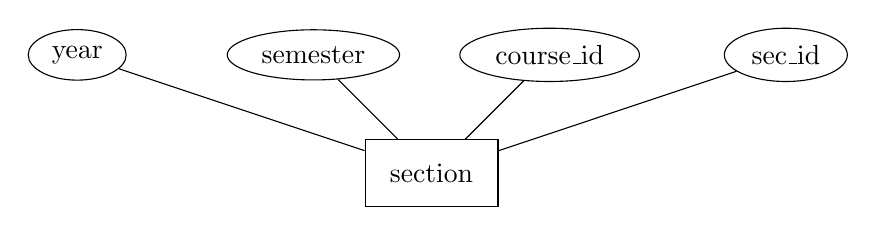
\begin{tikzpicture}[auto,node distance=1.5cm]
  % Create an entity with ID node1, label "Fancy Node 1".
  % Default for children (ie. attributes) is to be a tree "growing up"
  % and having a distance of 3cm.
  %
  % 2 of these attributes do so, the 3rd's positioning is overridden.
  \node[entity] (node1) {section}
    [grow=up,sibling distance=3cm]
    child {node[attribute] {\code{sec\_id}}}
    child {node[attribute] {\code{course\_id}}}
    child {node[attribute] {\code{semester}}}
    child {node[attribute]{\code{year}}};
\end{tikzpicture}
}

A \textbf{weak entity set} is one whose existence is dependent on another entity, called its \textbf{identifying entity}, the part of the primary key of this entity set is the primary key of the entity set it depends on as a \textbf{discriminator}. An entity set that is not a weak entity set is termed a \textbf{strong entity set}. Every weak entity must have a entity set it \textbf{existently depends} on.\\

In ER diagrams, a weak entity set is depicted via a double rectangle. Its discrimanotrs are underlined.\\

[Weak entity sets are simply entity sets that are dependant on other entity sets to exist.]

\section{Reducing ER Diagrams to Relational Schemas}

As a first approximation:

\begin{enumerate}
\item Turn each entity set into a relation with the same set of attributes.
\item Replace a relationship set by a relation whose attributes are the keys for the connected entity sets (and any descriptive attributes of the relationship sets).
\end{enumerate}

Weak entity sets change this somewhat.

\subsection{Representing entity sets}.

A strong entity set reduces to a schema with the same attributed, ie: A student entity set with attributes ID, name, and tot\_cred becomes \textit{student(\underline{ID}, name, tot\_cred)} A weak entity set becomes a table that includes a column for the rpimary key of the identifying strong entity set.\\

Composite Attributes are represented by dividing each composite part to normal attributes. [Composite attributes reduce to their subattributes.] Derived attributes are omitted completely.

Multivalued attributes map to brand new schemas, whose members are multiple values these attributes take. For instance, a student with a multivalued key phone number, maps to a phone number schema, whose members are all student's phone numbers, where a student may have multiple of them.\\


Many-to-one and one-to-many relationship sets that are total on the many-side can be represented by adding an extra attribute to the many side, containing the priamry of the one side. In one-to-one relationships, any side can be chosen as the many, albait, if the participation is not total, \code{NULL} values will occur.\\

Relations between weak entity sets and their corresponding strong entity sets are omitted as well, since they become redundant.

\subsection{Specialization}

Specialization is special entity set structure where a (weak) entity set is used as a subclass-like structure of another entity set. It can be overlapping (entity may occur in multiple specializations) or it may be disjoint, where this cannot occur.\\

Specializations are represented in schemas by creating a schema for the higher level entity, and then forming another schema for each lower-level entity set, include the primary key of the higher level entity set. Another method is to form a sechema for each entity set and include all local and inherited values. The drawback in the first is more queries being spent to look for a single entities records, and the for the second method more space being taken redunantly.\\

\subsubsection{Completeness Constraint}

Completeness constraint state wheter or not each entity in the higher level set must belong to a lower level entity set. Total Completeness means that it must, and Partial means it is not a must. The partial generalization is the default, when denoting a total generalization, a dashed line is drawn from the arrow, and on it the word \textit{total} is written.

\section{Design Problems}

There are certain design problems that may occur while designing a database system.

\subsubsection{Entities vs Attributes}

Certain attributes may be converted to entities on their own right if one wishes to store additional information about a specific attribute.

\subsubsection{Entities vs Relationship}

A guidline in deciding wheter or not something is an entity or a relationship is by asking if it is an \textit{actions}. Actions that occur between two of entities are relationships. Arguments directly related to relationships must become relationship attributes.

\subsubsection{Redunantant Atttributes}

Avoid repeating information. ER Diagrams \textit{are not} schemas, foreign keys are not needed to be shown if there is a relationship between them instead.

\chapter{Database Theory for Relational Databases - November 19, 2020}

\section{Features of Good Relational Design}

In a database we talked about the previous section, \code{instructor(ID, name, dept\_name, salary)} and \code{department(dept\_name, building, budget)} was two different schemas in this database. If we were to combine these two schemas into a relation, there would be a repetition of information, since instructors of the same departments will write budget data more than once. It also introduces the need to use \code{null} values, (if one adds a new department with no instructors.)\\

This is because, for this example, keeping two different tables is good. But in some cases, for instance \code{employee(ID, name, street, city, salary)} schema, decomposed into \code{employee1(ID, name)} and \code{employee2(name, street, city, salary)}, it might be impossible to reconstruct the original employee relation if more than one employee with the same name exists. These sorts of decompositions are called \textbf{loosy decomposition}. While a decomposition that can be reconstructed back to its original form is a \textbf{loseless composition}.\\

In conclusion, for the decomposition of a relation of $R$ to $R_1$ and $R_2$, if $R_1 \join R_2 = R$ it is lossless, otherwise, lossy.

\subsection{Functional Dependencies}

Suppose a schema of \code{Student(SSN, SName, address, HScode, HSname, HScity, GPA, priority)} suppose that the \code{priority} is determined by the \code{GPA}. If \code{GPA> 3.8, priority = 1}, \code{3.3 < GPA <= 3.8, priority = 2} and \code{GPA <= 3.3, priority = 3}. It can be concluded that \textit{two tuples with the same GPA have the same priority}.\\

$\forall t, u \in \code{student}: t\code{.GPA} = u.\code{GPA} \Rightarrow t\code{.priority} = u\code{.priority}$ Then, it is said that $\code{GPA} \rightarrow \code{priority}$ (\code{priority} is functionally dependent on \code{GPA}).\\

In general:

\begin{multline}
\text{if } \forall t, u \in R, t[A_1, A_2, \hdots, A_n] = u[A_1, A_2, \hdots, A_n] \\ \rightarrow t[B_1, B_2, B_m] = \\u[B_1, B_2, \hdots, B_m] \text{ then } A_1, A_2, \hdots, A_n \\\rightarrow B_1, B_2, \hdots, B_m
\end{multline}

$X \rightarrow Y$ is an assertion about a relation $R$. By convention, $X, Y, Z$ represets sets of attributes, $A, B, C$ represents sinlge attributes, and by convention $\{A, B, C\}$ may be written as $ABC$.

\subsection{Rules for Functional Dependencies}

\subsubsection{Splitting Right Sides of FDs}

if $X \rightarrow A_1 A_2 \hdots A_n$ holds for $R$ exactly when each of $X \rightarrow A_1, X \rightarrow A_2, \hdots X \rightarrow A_n$ hold for $R$, in general:

\begin{align}
A \rightarrow BC \Rightarrow A \to B \land A \to C
\end{align}

\subsubsection{Combining Rule}

The inverse of the splitting rule.

\begin{align}
A \rightarrow B \land A \Rightarrow C \Rightarrow A \to BC
\end{align}

\subsubsection{Triviality}

$X \to Y$ is a nontrivial functional dependency if $Y \nsubseteq X$ otherwise, it is a trivial functional dependency. Moreover, if $X \to Y$ is a \textbf{trivial functional dependency} then $X \to X \cup Y$ and also $X \to X \cap Y$.

\subsubsection{Transitivity of FDs}

If $X \to Y$ and $Y \to Z$, then $X \to Z$.

\subsubsection{Closure of Attributes}

The set of \textbf{all} functional dependencies logically implied by $X$ is the closure of $X$, given relation, a set of FDs, a set of attributes $X$, find $Y$ suvh that $X \to Y$.\\

The algorithm used for this purpose, starts with a set of attributes $X$, and a set of FDs of relation $R$. The closure $X^+$:

\begin{itemize}
\item If necessary, split the FDs of the $R$, so each FD in $R$ has a single attribute on the right.
\item Start with the set itself.
\item Repeat until there is no change. If $X \to Y$ and $X$ is in the set, then add $Y$ to the set.
\end{itemize}

For instance, given FDs $A \to B$ and $B \to D$, closure of $A$ evolves as:

\begin{itemize}
\item $A^+ = \set{A}$
\item $A^+ = \set{A, B}$
\item $A^+ = \set{A, B, D}$
\end{itemize}

\subsection{Keys of Relations}

$K$ is a \textbf{superkey} if they functionally determnie all other attributes. In other words, if $K^+ = X$ where $X$ is all attributes of $R$, then $K$ is a \textbf{superkey}.\\

Consider in scheme \code{Customers(name, addr, drinksLiked, manf, favDrink} if $\code{name} \to \code{addr, favDrink}$ and $\code{drinksLiked} \to \code{manf}$, here $\set{\code{name, drinksLiked}}$ is the superkey since its closure is all the attributes of the relation and also since its closure is all attrbiutes.\\

A key is a superkey if none of its strict subsets is also a superkey. Also consider that all of the supersets of a superkey is a superkey itself.\\

\subsection{Projecting Functional Dependencies}

\textbf{Normalization} refeers to the process where one breaks a relatino schema into two or more schemas, imagine a relation $R$ of attributes $ABCD$, with FDs $AB \to C, C \to D$ and $D \to A$. If one decomposes $R$ into $ABC, AD$ not only will $AB \to C$ will hold, but also $C \to A$.\\

Start with given FDs and find all \textit{nontrivial} FDs that follow from the given FDs, then restrict to those FDs that involve only attributes of the projected schema.\\

With inputs of two relationships $R, R_1$ where $R_1$ is decomposed from $R$, a set of FDs that hold in $R$.

\begin{enumerate}
\item Let $T$ be the eventual output set of FDs, initally, it is empty.
\item For each set of attributes $X$ that is a subset of atrributes of $R_1$, compute $X^+$
\item Add to $T$ all nontrivial FDs $X \to A$ such that $A \in X^+$ and an attribute of $R_1$.
\item However, drop from $T$, $XY \to A$ whenever we discover $X \to A$, because $XY \to A$ follows from $X \to A$ in any projection.
\item Finally use these FDs.
\end{enumerate}

There are a few tricks here, one does not need to compute the empty set an its closure, and if $X^+$ determines all attributes, then so does its supersets.\\

\subsubsection{Example}

For instance to $R(ABCD)$ FDs $A \to B, B \to C, C \to D$ project onto $R_1(ACD)$, we start from singletons and move onto biggers subsets. 

\begin{itemize}
\item $A^+ = ABCD$, thus $A \to C$ and $A \to D$ holds in $R_1$, note that $A \to B$ is true in $R$ but makes no sense in $R_1$. Since $A^+$ includes all attributes of $R_1$, there is no need to consider the supersets of $A$. 
\item $C^+ = CD$, thus $C \to D$ holds in $R_1$.
\item $D^+ = D$ is trivial, and yields no nontrivial FDs.
\end{itemize}

Thus, FDs for $R_1$ are $A \to C$ and $C \to D$, and of course, $A \to D$ from the transitivity rule.\\

[So \textit{that} is why they thought us predicate logic in Discrete Structures...]

\section{Anomalies}

Problems that arise in databases due to poor design are called \textbf{anomalies}.

\begin{description}
\item[Redundancy] Repeated information in several tuples.
\item[Update Anomalies] When a change in one ypule leaves the same inforamtion unchanged in another tuple.
\item[Deletion Anomalies] Losing information when deleting.
\end{description}

Consider for the schema \code{Customers(name, addr, drinksLiked, manf, favDrink}, if a customer likes more than one drink, the \code{favDrink} and \code{addr} will repeat unncesserilly.\\

Moreover, this bad design is also open to update and deletion anomalies. Consider, if a customer changes their address, what if the programmer does not remember updating all tuples containing them; or if no one likes coke, one loses track of the fact that Coca-Cola manufactures Coke.

\section{Boyce-Codd Normal Form}

The goal of decomposition is to replace a relation (that exhibits some anomalies) with several relations that do not exhibit anomalies.\\

The condition under which the anomalies discussed can be guranteed not to exist is called Boyce-Codd Normal Form, or BCNF.\\

We say $R$ is in BCNF if whenever $X \to Y$ is a nontrivial FD that holds in $R$, $X$ is a superkey.\\

In \code{Customers(name, addr, drinksLiked, manf, favDrink}, FD's are $\code{name} \to \code{addr favDrink}, \code{drinksLiked} \to \code{manf}$. Since \code{name} is not a superkey but appears in a FD, it violates BCNF.\\

Now consider \code{Customers(name, manf, manfAddr)}, FDs are $\code{name} \to \code{manf}$ and $\code{manf} \to \code{manfAddr}$, here the second FD violates BCNF.\\

We can replace an $R$ that is not in BCNF with two schemas:

\begin{enumerate}
\item $R_1 = X^+$
\item $R_2 = R -(X^+ - X)$
\end{enumerate}

And then projecting $R$'s FDs onto $R_1$, $R_2$.\\

\subsubsection{Example}

For instance, in \code{Customers(name, addr, drinksLiked, manf, favDrink}, and \fd{name}{addr}, \fd{name}{favDrink} and \fd{drinksLiked}{manf}.

\newcommand{\customersm}{\code{Customers(name, addr, drinksLiked, manf, favDrink)}}
\newcommand{\customerso}{\code{Customers1(name, addr, favDrink)}}
\newcommand{\customerst}{\code{Customers2(name, drinksLiked, manf)}}

\begin{itemize}
\item Pick BCNF violation \fd{name}{addr}
\item Close the left side: $\set{\code{name}}^+ = \set{\code{name}, \code{addr}, \code{favDrink}}$
\item This yields two decomposed relations \code{Customers1(name, addr, favDrink)} and \code{Customers2(name, drinksLiked, manf)}.
\end{itemize}

Now, check if \code{Customers1} and \code{Customers2} is in BCNF.

\begin{itemize}
\item If we get the closures for Customers1, $\code{name}^+ = \set{\code{name}, \code{addr}, \code{favDrink}}$, $\code{addr}^+ = \set{\code{addr}}$, $\code{favDrink}^+ = \set{\code{favDrink}}$. Only relevant FD (nontrivial ones) is \fd{name}{addr} and \fd{name}{favDrink}, which is in BCNF since \code{name} is a superkey.

\item But, Customer2, \customerso \textbf{does} violate VCNF, since the only nontrivial fd is \fd{drinksLiked}{manf} but \code{drinksLiked} is not a superkey by itself.
\end{itemize}

We decompose Customers2 to \code{Customers2(drinksLiked, manf)} and \code{Customers4(name, drinksLiked)}. The resulting decomposition of \customerst is:

\begin{itemize}
\item \code{Customers1(\emph{name}, addr, favDrink}, which telss us about customers
\item \code{Customers3(\emph{drinksLiked}, manf)} which tells us about drinks.
\code{Customers4(\emph{name}, \emph{drinksLiked})} which tells us about the relationship between customers and the drinks they like.
\end{itemize}

\section{3\textsuperscript{rd} Normal Form}

There is a possibly, when, decomposing a relation, because not all FDs are carried onto all decomposed relations, it is possible that, although no relations violate their own FDs, the database as a whole may violate one of the original FDs.\\

The 3\textsuperscript{rd} Normal Form (3NF) modifies BCNF to fix this issue. An attribute is called \textbf{prime} if it is a member of any key. $X \to A$ violates 3NF if and only if $X$ is not a superkey, and also $A$ is not a prime.\\

There are two important properties of a decomposition:

\begin{enumerate}
\item \textbf{Lossless Join} it should be possible to project the orignal relations onto the decomposed schema, and then rebuild them.
\item \textbf{Dependency Preservation} It should be possible to check in the projected relations wheter all FDs hold.
\end{enumerate}

BCNF does not preserve dependencies all the time, 3NF is a weaker normal form that allows some redunancy but also gurantees dependency preservation. It also gurantees lossless join.\\

In 3NF, the need for null values may arise from time to time, and there is also a problem of repetition of information.

\subsubsection{3NF Synthesis Algorithm}

There is a need for \textbf{minimal basis} for FD, a minimal basis  for FDs are:

\begin{enumerate}
\item Right sides are single attributes.
\item No FDs can be removed.
\item No attribute can be removed from a left side.
\end{enumerate}

To get a minimal basis:

\begin{enumerate}
\item Split right sides.
\item Repeatedly try to remove an FD and see if the remaining FDs are equivalent to the original.
\item Repeatedly try to remove an attribute from a left side and see if the resulting FDs are equivalent to the original.
\end{enumerate}

Then, we can create schemas by giving one relation for each FD in the minimal basis. Schema is the union of the left and right sides. And also, if none of them are a key, also the key for a relation.\\

In a relation $R=ABCD$, FDs are $A \to B$ and $A \to C$, and then $AB$ and $AC$ relations are decomposed from FDs, plus $AD$ for a key.

\chapter{Design Theory for Relational Databases (Cont`d) - November 16, 2020}

\newcommand{\C}[1]{\code{#1}}
\newcommand{\ApplyExample}{\C{Apply(SSN, cName, hobby)}}
Imagine a system with the relation \C{Apply(SSN, cName, hobby)}, we have no Functional dependencies for this relation, the only key is the all attributes of the relation. The relation is in the BCNF.\\

Is this a good design to hold student collage applications? Imagine a database such as:
\begin{table}[h]
    \begin{tabular}{lll}
		SSN & cName & Hobby\\
        \toprule
        123 & IYTE & tennis\\
        123 & IYTE & swimming\\
        123 & EGE & tennis\\
        123 & EGE & swimming\\
        \bottomrule
    \end{tabular}
    \caption{Instructors.}
    \label{tab:inst}
\end{table}

Sweet Jesus, this is terrifying, look at this monstrosity, if a student with 4 hobbies applies to 5 collages, that would create 20 tuples alone! This is a terrible design.

\section{Multivalued Dependency}

\begin{description}
\item[a Multivalued Dependency] (MVD) on $R$, denoted $X \to \to Y$ says that if two tuples of $R$ agree on all attributes of $X$, then their components in $Y$ may be swapped and the result will be two tuples that are also in the relation.
\end{description}

\newcommand{\mvn}{\ensuremath{\to\to}}
For instance, $\C{SSN} \mvn \C{cName}$, we swap collage names wherever the \C{SSN} of th e student is the same, and the resulting tuples will also be in the relationship.\\

For instance in \C{Customers(name, addr, phones, drinksLiked)}, here \C{phones} and \C{drinksLiked} are independent, which will create redundant tuples, we can just say $\C{name} \mvn \C{phones}$ and $\C {name} \mvn \C{drinksLiked}$.

\subsubsection{Every FD is an MVD}

Keep in mind that every Functional Dependency is a Multivalued Dependency as well. If $X \to Y$, then by definition $X \mvn Y$, since swapping $Y$s between two tuples that agree on $X$ doesn't change the tuples.

\subsubsection{Complementation}

If $X \mvn Y$, and $Z$ is all the other attributes $X \mvn Z$.\\

For instance, in the \ApplyExample, since $\C{SSN} \mvn \C{cName}$, automatically $\C{SSN} \mvn \C{hobby}$. [Since swapping \C{cName} values is equal to swapping \C{hobby} values in reverse.]

\subsubsection{Splitting Doesn't Hold}

Like the FDs, left side of an MVD cannot be generally split. \textbf{Unlike} FDs, the right side cannot be split either. If $A \mvn CD$, \textit{does not necessarily mean} $A \mvn C$ and $A \mvn D$.

\section{the Fourth Normal Form}

The Separation of independent facts is what 4NF is about. The redundancy that comes from MVNs cannot be fixed with BCNF. 4NF treats MVDs as FDs while decomposition.\\

A relation is in 4NF if: whenever $X \mvn Y$ is a nontrivial MVD, then $X$ is a superkey. Nontrivial MVD means that:

\begin{enumerate}
\item Y is not a subset of X.
\item X and Y are not, together, all the attributes.
\end{enumerate}

Superkeys are still determined by FDs only.\\

\subsubsection{Connection to BCNF.}

Since every FD is an MVD, if $R$ is in 4NF it is certainly BCNF, but R could be in BCNF and not in 4NF.\\

If $X \mvn Y$ is a 4NF violation for relation $R$, we can decompose $R$ using the same technique for BCNF.

\subsubsection{Algorithm.}

Until all relations are in 4NF:

\begin{itemize}
\item Pick any $R'$ with nontrivial $X \mvn Y$ that violates 4NF.
\item Decompose $R'$ into $R_1(X, Y) and R_2(X, \text{rest})$.
\item Compute FDs and MVDs for $R_1$ and $R_2$.
\item Compute keys for $R_1$ and $R_2$. 
\end{itemize}

\subsubsection{Example}

\newcommand{\mvd}{\mvn}

In the \ApplyExample, MVDs are:

\begin{enumerate}
\item $\C{SSN} \mvd \C{cName} $
\item $\C{SSN} \mvd \C{hobby}$
\end{enumerate}

The key is $\set{\C{SSN}, \C{cName}, \C{hobby}}$ and all dependencies violate 4NF.\\

The MVN (1) and (2) violates 4NF because $\C{SSN}$ is not a superkey.\\

Decompose using $\C{SSN} \mvd \C{cName}$:

\begin{enumerate}
\item \C{Apply1(\emph{SSN}, \emph{cName)}}, no MVDs or FDs, and in 4NF.
\item \C{Apply2(\emph{SSN}, \emph{hobby})}, no MVDs or FDs, and in 4NF.
\end{enumerate}

\part{Structured Query Language}

\chapter{SQL - November 26, 2020}

This chapter is the start of an overview of the \textbf{Structured Query Language}, SQL. [A declarative language, semi-standardised in ISO/IEC 9075] More specifically, the dialect of SQL used in the Oracle Database Systems.\\

Most (if not all) SQL statements can be among all dialects, and even when one-to-one compatibility is unavailable

\section{Statements}
\subsection{Select Statement}
Used to guery tables:
\begin{lstlisting}
SELECT * FROM dept;
SELECT deptno, loc FROM dept;
SELECT ename, sal, sal+300 FROM emp;
\end{lstlisting}

Here, \C{SELECT} is used to query the table denoted by \C{FROM}, \C{SELECT} statement is followed by the column names (seğerated by commas) that are wished to be retrieved.\\

Using the \C{*} sign will select all the columns.

Observe that by using arithmetic operations, we are able to view manipulated data as well. Keep in mind that \C{sal+300} \textbf{does not} change the table itself.

\subsubsection{Operator Precedence}

Operator precedence follows normal precedence rules, parenthesis maybe used to clarify precedence when need be.

\subsubsection{Null Values}

\C{NULL} values in are values that do not exist, they are not zero. They may also create problems in arithmetic operations, returning \C{NULL} themselves.

\subsubsection{Column Aliases}

\begin{lstlisting}
SELECT ename as name FROM emp;
SELECT ename "Name" FROM emp;
\end{lstlisting}

\C{AS} keyword is optional, an alias may follow the column name itself. But without double quotations, the entire word will be capitalised.

\subsubsection{Duplicate Rows}


\begin{lstlisting}
SELECT deptno FROM emp;
SELECT DISTINCT deptno FROM emp;
\end{lstlisting}

By default, queries will display the duplicate rows also. The, \C{DISTINCT} keyword can be used to get rid of these.

\subsubsection{Limiting Rows}

\begin{lstlisting}
SELECT ename, job, deptno 
FROM emp 
WHERE job='CLERK';

SELECT ename, job, deptno 
FROM emp
WHERE sal<=comm;
\end{lstlisting}

The \C{WHERE} clause is an optional clause that be used to filter rows. Observe that the \C{WHERE} clause can also be used with comparison operator. Do keep in mind that \C{NULL} values return \C{NULL} here too.

\begin{lstlisting}
SELECT ename, job,
	deptno FROM emp WHERE
	sal BETWEEN 1000 and 2000;
SELECT ename FROM
	emp WHERE mgr
	IN(7902, 7566, 7788);
SELECT ename FROM
	emp WHERE ename
	LIKE '_A%';
SELECT  ename, mgr
	FROM empt WHERE
	mgr IS NULL
\end{lstlisting}

\newcolumntype{L}[1]{%
  >{\raggedright\let\newline\\\arraybackslash\hspace{0pt}}p{#1}%
}

\begin{table}[h]
    \centering
    \begin{tabular}{L{3cm} L{3cm}}
		& Function\\
        \toprule
        \C{BETWEEN ... AND} & Return True values between two values.\\
        \C{IN(LIST)} & Return True if values in a list.\\
        \C{LIKE} & Pattern matching, \% denotes zero or many, \_ denotes one character.\\
        \C{IS NULL} & Returns True if value is \C{NULL}\\
        \bottomrule
    \end{tabular}
    \caption{Other Comparison Operators}
    \label{tab:inst}
\end{table}

Pattern matching characters can be combined, in the example above, names of the employees whose name start with a single character, than an M, and then one or more characters will return.\\

Furthermore, logical operators \C{AND}, \C{OR} and \C{NOT} is defined in SQL.



\subsubsection{Character Strings and Dates}

Character strings and date values are represented via single quotation marks! They are case sensitive. Column names, clauses, table names are \textbf{not} case sensitive.\\

Date format is DD-MM-YYYY by default.

\subsubsection{ORDER BY Clause}

The order of rows returned in a query result is undefined, \C{ORDER BY} clause, alongside the \C{ASC} (default) and \C{DESC} keywords can be used to order the rows of a query result.

\begin{lstlisting}
SELECT ename, job,
	deptno FROM emp
	ORDER BY hiredate DESC;
SELECT ename, job, deptno,
	sal*12 annsal
	FROM emp ORDER BY annsal;
\end{lstlisting}

As can be seen in the second example, column aliases can be used to order clauses as well.\\

\begin{lstlisting}
SELECT ename, job, deptno
FROM emp 
ORDER BY deptno, sal DESC;
\end{lstlisting}

Multiple columns can be sorted, the order of \C{ORDER BY} list is the order of the sort, the first option is sorted first, and if they are equal, \textbf{then} the second column is used, and so forth. One can also sort by a column that is not in the \C{SELECT} list.

\chapter{SQL (Cont`d) - December 3, 2020}

\section{Single Row Functions}

\subsubsection{Case Conversion Functions}

Consider
\begin{lstlisting}
SELECT ename, job,
FROM emp
WHERE ename = 'blake';
\end{lstlisting}

However, this will return nothing, since all of the employee names are in capital letters, we can use \C{UPPER} to account for this.

\begin{lstlisting}
SELECT ename, job,
FROM emp
WHERE ename = UPPER('blake');
\end{lstlisting}

There are other functions of this sort, such as \C{CONCAT(str, str)}, \C{LENGTH(str)}, \C{SUBSTR(str, start, stop)} that can be used for numerous purposes.

\subsubsection{Arithmetic Operators with Dates}

\begin{lstlisting}
SELECT ename, 
	(SYSDATE - hiredate)
	/7 WEEKS,
FROM emp;
\end{lstlisting}

As you we can see, the arithmetic operations work with date types.

\section{Multiple Tables}

So far, we only worked on a single table at a time, however, queries can be run on multiple tables, easily.

\subsection{Join}

\begin{lstlisting}
SELECT 	table1.column, table2.colum
FROM	table1, tabl2
WHERE	table1.column1 = table2.column2;
\end{lstlisting}

Column names are prefixed with the table name.

\subsubsection{Equijoin}

\begin{lstlisting}
SELECT 	emp.empno, emp.ename, emp.deptno
		dept.deptno, dept.loc
FROM	emp, dept
WHERE	emp.deptno=dept.deptno
\end{lstlisting}

\subsubsection{Joining More Than Two Tables}

If we have \C{employee(\emph{person-name}, street, city)}, \C{works(\emph{person-name}, company-name, salary)}, \C{company(\emph{company-name}, city)} and \C{managers(\emph{person-name}, manager-name)}. If we wish to find the names of all employees who live in the same city as the company for which they work.

\begin{lstlisting}
SELECT 	e.person-name
FROM	employee e, 
		works w, company c
WHERE	e.person-name 
		= w.person-name
	AND w.company.name = 
		c.company-name
	AND e.city = c.city
\end{lstlisting}

Here we joined three tables to achieve our task! [Observe that the aliases can be used in the \C{FROM tab}]. [I also like how we can use aliases \textit{before} we declare them, this means SQL as a language necessitates a two-pass compiler at least! (Like most languages, honestly, except C, but hey, that's C for ya.)]

\subsubsection{Non-Equijoins}

Joins do not need equalities to work. Non-Equijoins are joins that do not rise from equalities.

\begin{lstlisting}
SELECT 	e.name, e.sal, s.grade
FROM	emp e, salgrade s
WHERE	e.sal
BETWEEN s.losal AND s.hisal
\end{lstlisting}

\subsubsection{Outer Joins}

If a row does not satisfy a join condition, the row will not appear in the query results. One can use the outer join to also see rows that do not usually meet the join condition.

\begin{lstlisting}
SELECT 	table1.column, table2.column
FROM	table1, table2
WHERE	table1.column(+) = table2.column;
\end{lstlisting}

The side with the \textit{missing information} is given the outer join [unary postfix] operator \C{(+)}. [The fact that it is unary and postfix is not related, but you do not get the chance to see a unary postfix operator a lot of times, I \textit{had} to point it out.]

\subsubsection{Self Joins}

Joining a table to itself is called a self join. In the \C{EMP} table, each employer has a manager, but managers are also employees! (So they are in the same table)

\begin{lstlisting}
SELECT 	worker.ename 
		||' works for '
		||manager.ename
FROM	emp worker, emp manager
WHERE	worker.mgr, manager.empno;
\end{lstlisting}


\section{Group Functions}

Group functions operate on sets of rows to give one result per group. Such as the maximum value of a field in a table\\

Group functions include \C{AVG}, \C{COUNT}, \C{MAX}, \C{MIN}, \C{STDDEV} all group functions except \C{COUNT(*)} ignore \C{NULL} values. Group functions are used as \C{function\_name(column\_name)}.

They include:

\begin{table}
\begin{tabular}{ll}
& Meaning\\
\toprule
\C{AVG} & Average\\
\C{MIN} & Minimum\\
\C{MAX} & Maximum\\
\C{COUNT} & Number of rows\\
\C{NVL} & Include \C{NULL} values\\
\C{SUM} & Sum of Numbers\\
\bottomrule
\end{tabular}
\caption{Some group functions.}
\label{tab:groupfunctions}
\end{table}

\C{COUNT}, when written without a column name, also includes the \C{NULL} values. \C{COUNT} can also be used with the \C{DISTINCT} keyword, such as \C{SELECT COUNT(DISTINCT colname)}, in this form, only the \textit{unique} rows shall be counted.\\

The \C{NVL(column\_name, assume)} function can be used to interpret \C{NULL} values as the \C{assume}, thus forcing group functions to include \C{NULL}.

\subsection{Creating Groups of Data}

Sometimes, a table may be needed to be divided into smaller groups. Perhaps we want to divide employees by their groups, then we want to get the average salary for each department.

\begin{lstlisting}
SELECT	col, groupf(col)
FROM	table
[WHERE	condition]
[GROUP BY	col]
[ORDER BY	col];
\end{lstlisting}

For instance, using this syntax our example can be calculated via:

\begin{lstlisting}
SELECT	deptno, AVG(sal)
FROM	emp
GROUP BY	deptno
\end{lstlisting}

Remember, any column not inside a group function in the \C{SELECT} clause, \textbf{must} appear inside the \C{GROUP BY} clause. \textit{However}, the column in the \C{GROUP BY} clause does not need to appear inside the \C{SELECT} clause, (albeit the results would lack meaning).

\subsubsection{Grouping by More Than One Column}

If we wish to sum salaries in the \C{EMP} table, for each job, grouped by their department, we can do this as follows:

\begin{lstlisting}
SELECT	deptno, job, sum(sal)
FROM	emp,
GROUP BY	deptno, job;
\end{lstlisting}

Order does matter here.

\subsubsection{Excluding Group Results}

The \C{HAVING} clause, places following the \C{GROUP BY} clause can be used to restrict the results to certain results meeting a condition.

\begin{lstlisting}
SELECT	deptno, max(sal)
FROM	emp,
GROUP BY	deptno
HAVING	max(sal)>2900;
\end{lstlisting}

Will only show the those departments whose maximum salary is greater than 2900.

\subsubsection{Nesting Group Functions}

Group functions can be nested to a depth of two.

\section{Subqueries}

Suppose that we have the quert, "Who has a salary greater than Jones'", we have, in fact a subquery of "What is Jones' query", and this query's result is used in the main query.

\begin{lstlisting}
SELECT	cols
FROM	table
WHERE	exr (SELECT cols
			 FROM table
			 WHERE exr)
\end{lstlisting}


For instance, for our original query.

\begin{lstlisting}
SELECT	ename
FROM	emps
WHERE	sal >
(SELECT sal
FROM emps
WHERE ename='JOHN')
\end{lstlisting}

The subquery is executed first, since its result is used in the main query. Subqueries can be \textbf{Single-Row}, \textbf{Multi-Row} and \textbf{Multi-Column}.\\

\C{ANY} and \C{ALL} operator can be used to distribute a logical condition to the results of a multiple-row subqueries.

\section{Manipulating Data}

\subsection{Adding a Row}

\C{INSERT} statement can be used to add one row at a time to a table.

\begin{lstlisting}
INSERT INTO
	dept (deptno, dname, loc)
VALUES
	(50, 'DEVELOPMENT', 'DETROIT');
\end{lstlisting}

Columns are listed optionally. If all values are provided in the default order of the columns in the table, a new entity with these values will be created.

\subsubsection{Inserting Rows with Null Names}

In the implicit method, simply omit the column from the column list, its value will be \C{NULL}. The explicit method is to specify the \C{NULL} value with the \C{NULL} keyword.

\subsubsection{Inserting Special Values}

There are certain special functions that can be used to insert special values, such as \C{SYSDATE} which returns the system date.

\subsubsection{Copying Rows}

Instead of using the values clause, by writing a subquery selecting rows from another table, one can copy rows from another table.

\subsection{Updating a Row}

The \C{UPDATE} statement can be used to update a row.

\begin{lstlisting}
UPDATE emp
SET	deptno = 20
WHERE empno = 7782
\end{lstlisting}

If one omits the \C{WHERE} clause, \textit{all} the rows will be modified. One-to-one matching between subqueries and queries can be used to update a table as well.

\subsection{Removing a Row}

the \C{DELETE} statement can be used to delete rows.

 \begin{lstlisting}
DELETE FROM	department
WHERE	dname='DEVELOPMENT';
\end{lstlisting}

Omitting the \C{WHERE} clause would delete all the rows of the table.

\section{\C{COMMIT} and \C{ROLLBACK} Statements}

\C{COMMIT} and \C{ROLLBACK} is used for the following purposes:

\begin{itemize}
\item Ensure data consistency.
\item Preview data changes before making changes permanent.
\item Group logically related operations.
\end{itemize}

Following a \textbf{Transaction}, one can \C{COMMIT} the transaction, making it permanent, or \C{ROLLBACK} back to a \textbf{savepoint} or to the last \C{COMMIT}\\

Please keep in mind that \C{COMMIT} and \C{ROLLBACK} is unusable in Oracle's Web-based Database Engine, as it auto-commits statements.

\subsubsection{State of the Data Before \C{COMMIT} or \C{ROLLBACK}}

\begin{itemize}
\item The previous state of the data can be recovered.
\item The \textit{current} user can review the results of the DML operations by using the \C{SELECT} statements.
\item Other users cannot interact with the changed rows, they are \textit{locked}.
\item Other users cannot see the changes, yet.
\end{itemize}

\subsubsection{State of the Data After \C{COMMIT}}

\begin{itemize}
\item Dta changes are made permanent.
\item The previous state of data is permanently lost.
\item All users can see the results.
\item Locks are released.
\item Savepoints are erased.
\end{itemize}

\subsubsection{State of the Data After \C{ROLLBACK}}

\begin{itemize}
\item All pending changes are discarded, data changes are undone.
\item The previous state of the data is restored.
\item Locks on affected rows are released.
\end{itemize}

\chapter{SQL (Cont`d) - December 17, 2020}

\section{Table Creation and Modification}

\C{CREATE TABLE} and \C{ALTER TABLE} statements can be used to create new tables and modify existing tables respectively.

\subsection{Table Creation}

The \C{CREATE TABLE} statement can be used to create a table in SQL.

\begin{lstlisting}
CREATE TABLE tableName
	(colName colType(colSize),
	colName2 colType(colSize),
	...
	);
\end{lstlisting}

\subsubsection{Data Types in Oracle SQL}

\begin{table}[h]
    \centering
    \begin{tabular}{l L{6cm}}
		Data Type & Description\\
        \toprule
        \C{VARCHAR2(size)} & Variable-length character data\\
        \C{CHAR(size)} & Fixed-length character data\\
        \C{NUMBER(p, s)} & Variable length numeric data\\
        \C{DATA} & Data and time values.\\
        \C{LONG} & variable-length character data up to 2GBs\\
        \C{CLOB} & Single-byte character data up to 4 gigabytes.\\
        \C{RAW}, \C{LONG RAW} & Raw binary data\\
        \C{BLOB} & Binary data up to 4 gigabytes\\
        \C{BFILE} & Binary data stored in an external file; up to 4GBs.\\
        \bottomrule
    \end{tabular}
    \caption{Data types in Oracle SQL, different SQL Dialects support different types.}
    \label{tab:datatypes}
\end{table}

\subsubsection{\C{CREATE TABLE} with a Subquery}

Using the \C{AS} keyword, \C{CREATE TABLE} can be used with a subquery. [Similar to piping output in Unix systems.], when getting data from another table this way, the constraints are preserved.

\subsection{Table Modification}

\C{ALTER TABLE} statement can be used in conjunction with the \C{ADD} and \C{MODIFY} keywords to add new columns or modify existing columns of a table.\\

The table modification can update the type of an existing column.

\section{Constraints}

During table creations, SQL can be used to add constraints to certain columns or tables. \textbf{Column-level constraints} are written after a column type/size in the table creation. Whereas, \textbf{Table-level constraints} are written after writing all the columns, the table-level constraints follow the \C{CONSTRAINT} keyword and may refer to multiple columns.

\subsubsection{the \C{NOT NULL} Constraint}

Ensures that \C{NULL} values are not permitted for the column. It \textit{cannot} be defined at the table level. [In fact, this behaviour is shared when checking for equalities. \C{NULL} does not equal to any value including another \C{NULL}, similar to the behaviour of \C{NaN} in IEEE 754.]

\subsubsection{the \C{UNIQUE KEY} Constraint}

Ensures that the column cannot hold the two (or more)  copies of the same value. Two values holding \C{NULL} \textit{can} be inserted. The \C{UNIQUE KEY} constraint can be defined at either the table level or the column level.

\subsubsection{the \C{PRIMARY KEY} Constraint}

This constraint acts both as a \C{NOT NULL} constraint and a \C{UNIQUE KEY} constraint. The values inserted at this column must be unique \textit{and} must not be \C{NULL}.


\subsubsection{the \C{FOREIGN KEY} Constraint}

The \C{FOREIGN KEY} constraint is used for columns that hold the values of a primary key of another table. It is sometimes refereed to as the Referential Integrity Constraint.\\

When a column is defined to be a \C{FOREIGN KEY}, the values it hold \textit{must} exist in the primary key of another table.\\

It has a unique syntax, and is used in conjunction with the \C{REFERENCES}.

\begin{lstlisting}
FOREIGN KEY (nativeCol)
REFERENCES foreignTable (foreignCol);
\end{lstlisting}

If followed by the \C{ON DELETE CASCADE}, should the row containing the primary key in the parent table is deleted, the records it references in the child table is deleted as well. It should be noted that, if not followed by this keyword, it won't be possible to delete the records whose referenced by other tables in the parent table. (\S\C{ORA-02292}).

\subsubsection{the \C{CHECK} Constraint}

Defines a condition that each row must satisfy.

\subsection{Constraint Modification}

Constraints may be added, or dropped; enable or disabled to a table using the \C{ALTER TABLE} constraint. If used in conjunction with the \C{ADD CONSTRAINT} keyword, it adds a constraint; if instead used with the \C{DROP CONSTRAINT} keyword, it drops a constraint instead.\\

\subsubsection{the \C{CASCADE} Constraint}

Using the \C{CASCADE} keyword following a \C{DROP CONSTRAINT} of a \C{PRIMARY KEY}, it also drops the \C{FOREIGN KEY} constraints associated with this column.\\

Attempting to drop a primary key constraint with foreign key constraints put on it from other tables without \C{CASCADE} will result in an error (\S \C{ORA-02273})\\

\subsubsection{Disabling and Enabling Constraints}

Primary keys can be activated or disabled using \C{DISABLE} and \C{ENABLE} keywords.

\subsubsection{Viewing Constraints}

Constraints can be viewed from the special table \C{user\_constraints} table. The columns associated with these constraints can also be viewed from the \C{user\_cons\_columns} special table.

\part{Databases}

\chapter{Integrity and Security in Databases - December 17, 2020}

\begin{description}
\item[Integrity] The database should not become incorrect or inconsistent to an inadvertent update (such as a typo)
\item[Security] The database should not be able to be reached by the unauthorised people.
\item[Constraint] The allowable states that the tables in the database may be in.
\end{description}

An \textbf{integrity constraint} encodes business rules about the organization. It can detect bad data entry, and it can enforce the rules of the organization. It may apply to an individual record, one or more table(s), or an entire database.\\
 
Consider \C{STUDENT(SId, SName, GradYear, MajorId)}. An integrity constraint may be that the \C{GradYear} must at least be \C{1863}. Another rule may be that "A professor teaches at most two sections a year" \C{SECTION(SectId, CourseId, Prof, YearsOffered)}, applies to this table as a whole. A constraint such as "a student cannot take a course more than once", applies to multiple tables simultaneously.\\

\C{CREATE TABLE} can only be used to specify a fraction of possible integrity constraints. Only those that apply to the individual records in a table. One needs to use \textbf{assertions} if they wish to have more complex constraints.

\begin{lstlisting}
create assertion SmallSections
check (not exists
	select e.SectionId
	from ENROLL e
	group by e.SectionId
	having count(e.EId) > 30)
\end{lstlisting}

Here, we can see the Standard SQL specification of the integrity constraint "No section can have more than 30 students". An Assertion can denote any constraint whose violation can be expressed as a query.\\

The \C{NOT EXISTS} operator returns true when a query returns no records.\\

\section{Triggers}

Oracle SQL \textbf{does not have} a \C{CREATE ASSERTION} statement. Instead, it has \textbf{Triggers}. A trigger specifies an action that the database system invokes automatically whenever a specified event occurs. A trigger has three essential parts:

\begin{enumerate}
\item an \textbf{Event}, the update statement that initiates the activity.
\item a \textbf{Trigger}, the predicate that determines whether the trigger will fire.
\item an \textbf{Action}, what happens if the trigger does fire.
\end{enumerate}


THe Standard SQL defines triggers as:

\begin{lstlisting}
CREATE TRIGGER trigger_name
{BEFORE|AFTER} {INSERT|
		DELETE|UPDATE}
	[OF col_name] ON tablaName
[REFERENCING <old or 
	new values alias>]
[FOR EACH ROW]
[WHEN condition]
action
\end{lstlisting}

A trigger action is bracketed by the keywords \C{BEGIN} and \C{END}. The Oracle SQL defines triggers as:

\begin{lstlisting}
CREATE [OR REPLACE] TRIGGER trigger_name
{BEFORE|AFTER} {INSERT|DELETE|UPDATE}
	[OF col_name] ON tableName
[REFERENCING old as <oldrow>
	new as <newrow>]
[FOR EACH ROW]
[ENABLE/DISABLE]
[WHEN condition]
BEGIN
action statements
END
\end{lstlisting}

The oracle also defines \C{:new.column-name} and \C{:old.column-name} automatically without using \C{REFERENCING as well}. Triggers in Oracle SQL can also be disabled or enabled. Enabled triggers automatically fires, disabled triggers do not.\\

[It is a bit interesting that unlike other standardised languages, SQL Standard is not adhered to by its vendors. Although some variations exists in some standardised languages, the syntax deviations seen between different dialects of SQL is not seen in any other standardised language, neither in C, C++ or ADA, for instance.]

\subsection{Triggers and Constraints}

Both triggers and constraints can constraint data input, constraints are easier to write and less error-prone than triggers that enforce the same rules. A constraint rejects any update that violates it, when a trigger \textit{fixes} the bad update. Constraints are also less error prone, and one should prefer constraints whenever possible. But, some rules can only be conveyed properly by triggers

\section{Authorisation}

Constraints and triggers help keep the database from becoming accidentally corrupted. Now, we need to make sure that malicious users cannot corrupt the database intentionally or look at private data.\\

SQL acts on a system of privileges. Different users can have different privileges for specific tables. A statement such as \C{grant update on ENROLL to Einstein} gives the update privileges to the user Einstein.\\

\subsubsection{Roles}

SQL has a concept of roles. [Similar to Unix concept of a user group] A role, is a category of users, and privileges can be granted to a role as a whole.\\

For the syntactical purposes, the \C{GRANT} sees roles and users as the same. A user can be assigned multiple roles at the same time.The privileges of a user will be the union of the privileges of its roles.

\subsubsection{Column Privileges}

Privileges can also be assigned on a column-level, such as \C{GRANT SELECT (StudentId, Grade) on ENROLL to dean, professor}. The users with these rolls will be able to select these two columns on the \C{ENROLL} table specifically.\\

Users with the \C{update, insert} and \C{delete} privileges also need to have \C{select} privileges for the fields in the \C{WHERE} clause. They do not need this privilege if their query does not contain a \C{WHERE} clause.\\

\subsubsection{Granting Constraint Privileges}

The \C{grant reference} privilege, grants the privilege to create constraints on a table.

\subsubsection{Grant-Option Privileges}

The \C{with grant option} clause, added to the end of a \C{grant} statement gives the user who is granted a privilege the privilege to grant that same privilege to other users.

\subsection{Mandatory Access Control}

the SQL authorisation mechanism used by SQL is called \textbf{discretionary access control}. The creator of a table has authorisation on their tables, and may give access to others at his discretion.\\

A database system that uses discretionary access control depends on its users to be trustworthy. If a user is not trustworthy, the user can just copy information they have access to and release it to the public.\\

Contrasting with Discretionary Access Control, Mandatory Access Control assigns privileges to data, instead of tables. Each record and user is assigned to a classification level, a user is authorised to see a record if the user's classification level is equal or higher to the data's classification level.\\

This access control is predominantly used in high-security environments such as the military, and is not preferred in commercial settings.

\chapter{Views - December 24, 2020}

[Merry Christmas and Happy Hanukkah to any friends that may be reading this! (And Yule as well, 'suppose.) the Year is almost over, eh? I sure am happy that \textit{this} year is ending, let us hope for a better one for the next.]\\

In the first lecture, three schema levels, \textbf{Physical Schemas} (files, indexes), \textbf{Conceptual Schemas} (user-neutral data) and \textbf{External Schemas} (user-specific tables).\\

A \textbf{view} is essentially a named query, A user can refer to a view as if it were a table.

Views are useful for:

\begin{itemize}
\item Hiding some data from some users.
\item Making certain queries easier or more natural.
\item Increasing the modularity of database access.
\end{itemize}

\section{Virtual Views}

Virtual Views are the most often used [and historically the first] views. In this chapter, when the term view is used without any descriptive, it refers to a view.\\

View data is not stored on the disk, it is a \textbf{virtual relation} based on the result set of a \C{SELECT} statement. Views are customized presentations of data in one or more tables or other views, they can be thought of  as stored queries, they derive data from other tables.\\

Views in the Standard SQL and Oracle SQL can be created as follows [this paragraph is here just to pad the code example to the next column so it doesn't split and look ugly]

\begin{lstlisting}
CREATE VIEW view_name AS
SELECT column_name(s)
FROM table_name
WHERE condition;
\end{lstlisting}

[View performance is comparable to normal queries in Oracle DBMS, there is no difference since they are \textit{stored queries}. (\S9673409)) In Microsoft SQL, they are actually a bit faster due to caching (referred to as \textit{indexing}) (\S439061).]\\

Views can be created from two separate tables, by giving multiple tables in the \C{FROM} clause.\\


\subsubsection{Updatable Views}

A view is updatable if every record in the view has a unique corresponding record in some underlying database. In practice, this reefers to single-table view that do not involve aggregations, and multi-table views are \textit{in general} not updatable.\\

This problem arises from the fact that, when deleting (for instance) the system can delete the record from any of the tables constituting the table, this ambiguity leads to DBMS not allowing deletion altogether.\\

In conclusion, views that do not have one to one relationships such as due to multi-tables or aggregation functions (\S7.3).

\subsubsection{Inserting to Views}

When inserting new values, the constraints on the fields of the view rows must be taken into account, the said fields must be a part of the view since only then can we insert new values, (if the field is \C{NOT NULL} for instance, we need to specify its value) Therefore, just because a table is updatable does not mean it is (always) modifiable.

\subsubsection{\C{DROP}}

The \C{DROP VIEW} will drop the view itself, which can be done on any view whether or not it is updatable. It does not affect the underlying table.

However, using the \C{DROP TABLE} on the underlying table makes the view unusable, since the Views depend on their underlying tables for reference.

\subsubsection{Read Only Views}

\C{WITH READ ONLY} keyword, added to the end of a view declaration makes that view not updatable irregardless of the conditions of the tables creation.

\section{Materialised Views}

Materialised Views are a form of controlled redundancy. They are tables containing the outputs of a view, and unlike virtual views they are stored on disk, whenever the underlying data is updated, so should the corresponding materialised views.\\

In certain situations, Query Optimiser may decide to use a materialised view rather than the original table.\\

Materialising \textit{frequently-accessed} views whose outputs are  \textit{expensive to recompute} is beneficial, however it is a bad idea to materialise a table if it is \textit{frequently-updated} and has a \textit{large output}. \\

Rather than completely resetting the materialised view, the SQL systems generally incrementally update these views.\\

\subsection{Materialized Views in Oracle}

When a materialized view is defined, its refresh option can be specified. Either \C{ON COMMIT}, which refreshes one of the materialized view's fact tables commit. \C{ON DEMAND} uses a manual refresh action.\\

Furthermore, the what type of refresh is done can be specified. \C{COMPLETE} (Total redefining), \C{FAST} (Incremental), \C{FORCE} (Try fast refresh, if doesn't work apply apply a \C{COMPLETE} refresh.), \C{NEVER} (Oracle Refresh Mechanisms do not apply on the table).

\subsection{Why Use Materialised Views}

Not only does Materialised Views has all of the benefits of the normal Views, but they also \textbf{improve query performance}, if the workload is designed correctly.

\chapter{Transactions \& Recovery - January 7, 2021}

A transaction is a group of operations that behaves as a single operation, a transaction is seen as a cohesive unit from the outside but actually consists of multiple operations. \\

\section{Requirements}

There are certain requirements for a transactions. These are called ACID properties, and every DBMS that has transactions must guarantee these, somehow.

\subsubsection{Atomicity}

The transactions are \textbf{atomic}, if one operation of a transaction fails, none of the operations within a transaction will be reflected in the database.\\

Either all of its operations succeed (commit) or they fail (rollback).

\subsubsection{Consistency}

The \textbf{consistency requirement} says that the database must be consistent in the start and end of the transaction, but may be temporarily inconsistent during execution.\\

Every transaction leaves the database consistent.

\subsubsection{Isolation}
Since if another transaction is executing concurrently with a transaction it may see an inconsistent database, the \textbf{isolation requirement} says that a transaction should not be aware of other transactions.

A transaction behaves as if it is the only thing running on the system.

This can be trivially achieved by making transactions execute serially.

\subsubsection{Durability}

The \textbf{durability requirement} says that once the user has been notified that a transaction has been completed, the updates to the database by the transaction must persist even if there are software or hardware failures.

Changes made by a committed transaction are guaranteed to be permanent.

\section{Transaction}

A transaction is initiated either by a high-level data-manipulation language such as SQL, or by a programming language such as C++ or Java.\\

In SQL, the \C{BEGIN TRANSACTION} keyword starts a transaction, and a \C{COMMIT} keyword typically ends it.\\

Typically, multiple transactions are allowed to run concurrently in a system allowing better transaction throughput and reducing average response time for transactions, \textit{Concurrency control schemes} are necessary to achieve isolation.

\subsection{Schedules}

A \textbf{schedule} is a sequence of instructions that specify the chronological order in which instructions of concurrent transactions are executed.\\

A transaction that successfully completes its execution will have a commit instruction as its last statement, otherwise its last statement will be a rollback instruction.

\subsubsection{Serializability \& Conflicts}

A schedule is said to serialisable if it is equivalent to a serial schedule.

In the simplified view of transactions consisting of only write and read instructions, any pair of instructions $(I_i, I_j)$ where both of them refer to the same variable, if both are not read statements than they are conflicting.

If $I_j$ and $I_i$ are consecutive in a schedule and they do not conflict, they shall also not conflict if they are swapped, If a schedule $S$ can be transformed into a schedule $S'$ by a series of swaps of non-conflicting instructions, $S$ and $S'$ are \textbf{conflict equivalent}. If a schedule $S$ is conflict equivalent to a serial schedule, than they are \textbf{conflict serializable}.

\subsubsection{Precedence Graph}

A schedule with a set of instructions $T_1, T_2, ..., T_n$ A precendence graph is drawn whose nodes are transactions and whose edges arise when a conflict arise, the direction of an edge is determined from the transaction with preceding instruction.\\

A schedule is conflict serialisable if and only if its precedence graph is acyclic, if it is acyclic, the serialisable order is obtained by a topological sorting of the graph, a linear order consistent with the partial\\

\textbf{A schedule is correct only if it is conflict serialisable due to the isolation requirement of the ACID.}

\subsubsection{Recoverable Schedules}
Schedules must be recoverable to make sure that if transaction $A$ sees the effects of the transaction $B$, and $B$ is rolled back, then so should $A$.\\

A schedule is recoverable if two transactions $T_j$ and $T_i$, and $T_j$ reads data $T_i$ wrote, then $T_i$ s commit must occur first.\\

A cascading rollback occurs when rollback of one transaction triggers the rollback of another, these are undesirable since they lead to the undoing of significant amount of work, for each pair of transactions $T_i, T_j$ such that $T_j$ reads a data item previously written by $T_i$, the commit operation of $T_i$ appears before the read operation of $T_j$. This is called a \textbf{cascadeless schedule}, all cascadeless schedules are also recoverable schedules.

\subsection{Transaction Management}

A transaction starts by executing a \C{BEGIN TRANSACTION} operation and is terminated by a \C{COMMIT} or \C{ROLLBACK} operation, a \C{COMMIT} establishes as commit point and a \C{ROLLBACK} returns to the previous commit point.\\

Transaction managment primarily deals with Recovery and Concurrency.

\section{Recovery}

Recovery is the restoration of the database to a correct state after a failure has occurred. It is based on \textit{redundancy}, physical redundancy is desirable, logical redundancy is not. A recovery \textit{log file} keeps the previous and after state.\\

A recovery is performed each time the database system starts up, its purpose is to restore the database to a reasonable state.

\subsubsection{Reasonable State}

\begin{itemize}
\item All uncompleted transactions should be rolled back.
\item All committed transactions should have their modifications written to disk.
\end{itemize}


\subsection{Undo-Redo Recovery Algorithm}

One of the main algorithms, Undo-Redo Algorithm assumes that all updated records for an uncompleted transaction will be in the log file.\\

It \textbf{undoes} the modifications made by uncommitted transactions, and \textbf{redoes} the modifications made by committed transactions.

\subsection{Checkpointing}

Log file size will increase drastically with time, the recovery algorithms stops considering the logs when it reaches a checkpoint.

A checkpoint is taken by forcing the contents of the main-memory buffers out to the disk and forcing a special checkpoint record out to the log, it contains all transactions that were in progress at the time the checkpoint was taken.

\chapter{Concurrency - January 14, 2020}

In a multi-process environment multiple transactions may occur \textit{concurrently}, this however comes with three fundamental problems.\\

[Not all DBMS' allow concurrency, SQLite being the most notorious example of this, not allowing write concurrency and only allowing limited read concurrency.]

\begin{description}
\item[the Lost Update Problem:] A second transaction reads the state of the database prior to the first one writing a change and then stomps on the first one's change with its own update.
\item[the Uncommitted Dependency Problem:] A second transaction relies on a change that has not yet been committed and is rolled back after the second transaction has begun.
\item[the Inconsistent Analysis Problem:] An error that occurs when totals are calculated during interleaved updates.
\end{description}

\section{Conflicts}

If $A$ and $B$ are concurrent transactions problems can occur if $A$ and $B$ want to read or write the same database object tuple $t$.\\

A problem only arises if at least one of the transactions is a write, since two reads cannot interfere with each other.

\begin{table}
\begin{tabular}{lll}
\toprule
$A$ & $B$ & Problems\\
\midrule
Read & Write & Inconsistent Analysis\\
Write & Read & Uncommitted Change\\
Write & Write & Lost Update\\
\bottomrule
\end{tabular}
\caption{Types of conflicts and problems they cause.}
\label{tab:transactionconflict}
\end{table}

\section{Locking}

Transactions lock a portion of the database to prevent these problems, there are two types of locks:

\begin{description}
\item[Exclusive Lock (X)] Locked by writing transaction, locks all other transactions.
\item[Shared Lock (S)] Locked by reading transaction, disallows writes.
\end{description}

\begin{table}
\begin{tabular}{l|l|l}
\toprule
& S & X\\
\hline
S & true & false\\ \hline
X & false & false\\
\bottomrule
\end{tabular}
\caption{Lock matrix showing the compatibility of lock types.}
\label{tab:lockmatrix}
\end{table}

A transaction is granted a lock if and only if the requested lock is compatible with locks already on the item by other transactions, any number of transactions can hold shared locks on an item but only one can hold an exclusive lock (and if an item has an exclusive lock on it, it cannot have shared locks.)


\subsection{Locking Protocol}

Locks can be put using different protocols.

\subsubsection{Two-Phase Locking Protocol}

This protocol ensures conflict-serialisable schedules. It consists of two phases, the \textbf{Growing Phase}, where a transaction may obtain but may not release locks, and the \textbf{Shrinking Phase} where transaction may release but may not obtain locks.

\subsection{Deadlock}

The term \textbf{deadlock} refers to when two transactions acquire locks on items each other needs, making it impossible for the both to make progress.\\

This situation can occur in most locking protocols, it can be solved by rolling back and releasing the locks of either one of the deadlocked transactions.

\subsubsection{Starvation}

If a transaction is waiting for an X-lock on an item while a sequence of other transactions are requesting S-locks on the same item, the original transaction is repeatedly rolled backed due to deadlocks.\\

This is called \textbf{starvation}, and is the sign of a badly designed concurrency control manager.

\subsubsection{Deadlock Prevention Strategies}

\begin{description}
\item[Wait-Die] Transaction 2 waits if it is older than 1, otherwise it is rolled back.
\item[Wound-Wait] Transaction 2 rolls back transaction 1 if it is older.
\item[Timeout-Based] A transaction waits for a specified amount of time for a lock, starvation may occur.
\end{description}

The oldest transactions survives and the rolled back transaction is restarted with the original timestamp.

\subsubsection{Deadlock Detection}

A system must use a dadlock detection and recovery schemes, \textbf{wait-for-graph} represents vertices as transactions and edges as lock waiting, when a cycle occurs in this graph, it means a deadlock has occurred.

\section{Isolation}

Transactions are isolated to certain \textbf{Isolation Levels}.

\begin{description}
\item[Read Uncommitted] Uncommitted records may be read.
\item[Read committed] Only committed records can be read, but successive reads may return different values.
\item[Repeatable Read] Ensures that a read is repeatable throughout the transaction.
\item[Serialisable] Ensures serialisable execution.
\end{description}

As the level of isolation increases, the interference and the level of concurrency decreases.\\

These levels apply to \textbf{data reading} only.

Certain problems may arise in isolation.

\begin{description}
\item[Dirty Read] A transaction reads a value written by another transaction that hasn't been committed yet.
\item[Nonrepeatable read] A transaction reads the same object twice during execution and finds different values despite not changing it.
\item[Phantom Read] A transaction re-executes a query returning a set of roews that satisfy a search condition and finds that the set of rows satisfying the condition has changed as a result of another recently committed transaction.\end{description}

As the level of isolation increases, all these problems are tackled one by one.
\end{document}
